\documentclass[../Main/main.tex]{subfiles}


\begin{document}
	\graphicspath{{../Time dependent equations/figs/}}
	\chapter{Convergence of the MPFA-L Method for Richards' Equation}
	In this chapter we use the results from chapter three to prove convergence of the Richards equation discretized in space with MPFA-L method, in time with backward Euler and linearized with the L-scheme.
	We start by considering the Richards' equation without the gravity term in an isotropic medium: Find $\psi = \psi(x,t)$ such that
	\begin{equation}\label{eq:richards w bc}
		\left \{
		\begin{aligned}[c]
			\partial_t \theta(\psi) - \nabla \cdot \left (\kappa(\theta (\psi)) \nabla \psi \right ) &= f, \\
			\psi &= 0, \\
			-\kappa(\theta (\psi)) \nabla \psi &= g_N,\\
			\psi &= u_0,
		\end{aligned}
		\ \ \
		\begin{aligned}[c]
			\text{ in }& \Omega \times (0,T]\\
			\text{ on }& \partial \Gamma_D \times (0,T]\\
			\text{ on }& \partial \Gamma_N \times (0,T)\\
			\text{ on }& \Omega \times \left\{t=0\right \}
		\end{aligned}
		\right.
	\end{equation}
	This equation has a non linearity in the flux, $\bm{q}=-\kappa(\theta (\psi)) \nabla \psi$, which makes it hard to apply our results, as they require a homogeneous medium. The hydraulic conductivity, $\kappa(\theta (\psi))$, depends on our solution which is heterogeneous, and is thus itself heterogeneous.
	To remedy this we use the Kirchhoff transform 
	\begin{equation}
		\begin{aligned}
			\mathcal{K} :\mathbb{R} &\rightarrow \mathbb{R}^{+}\\
			\psi &\mapsto \int_{0}^{\psi} \kappa(\theta(\phi)) \ d \phi = u.
		\end{aligned}
	\end{equation}
	As discussed in \ref{sec:TwoPhase}, the functions $\theta(\cdot)$ and $\kappa(\cdot)$ are continuous, monotone increasing functions, the Kirchhoff transform, $\mathcal{K}$, therefore has an inverse, $\mathcal{K}^{-1}$. 
	We define
	\begin{equation}
		\begin{aligned}
			b(u) &:= \theta(\mathcal{K}^{-1}(u))\\
			k(u) &:= \kappa (\theta (\mathcal{K}^{-1}(u))).
		\end{aligned}
	\end{equation}
	Further, assume that the hydraulic conductivity is bounded below and above
	\begin{equation}
		0<\kappa_m \leq \kappa(\theta) \leq \kappa_M,
	\end{equation}
	and that the water content is a Lipschitz continuous function of pressure
	\begin{equation}
		sup_{\psi} |\theta(\psi)|\leq L_{\theta}.
	\end{equation}
	Then $b(\cdot)$ is also Lipschitz continuous
	\begin{equation}
		\sup_{u} |b'(u)| = \left |\theta'(\mathcal{K}^{-1}(u))\frac{1}{\mathcal{K}' (\mathcal{K}^{-1}(u))}\right| = \left  |\theta'(\mathcal{K}^{-1}(u))\frac{1}{\kappa (\mathcal{K}^{-1} (u))}\right|\leq L_B.
	\end{equation}
 	\par
	We note that we in fact remove the non linearity in the constitutive law; by the chain rule, we get
	\begin{equation}
		\nabla u = \kappa(\theta(\psi))\nabla \psi.
	\end{equation}
	We can write the Richards' equation \eqref{eq:richards w bc} in the transformed variable $u$ to get: Find $u=u(x,t)$ such that 
	\begin{equation}\label{eq:richards simple}
	\left \{
	\begin{aligned}[c]
		\partial_t b(u) - \nabla \cdot \nabla u &= f, \\
		u &= 0, \\
		-\nabla u &= g_N,\\
		u &= u_0,
	\end{aligned}
	\ \ \
	\begin{aligned}[c]
		\text{ in }& \Omega \times (0,T]\\
		\text{ on }& \partial \Gamma_D \times (0,T]\\
		\text{ on }& \partial \Gamma_N \times (0,T)\\
		\text{ on }& \Omega \times \left\{t=0\right \}
	\end{aligned}
	\right.
\end{equation}
We start by discretizing \eqref{eq:richards simple} with the MPFA-L method, we divide our domain into $d$ quadrilaterals (control volumes). Writing \eqref{eq:semidiscrete FVM} in vector form we find $\tilde{u}_h \in \mathbb{R}^d$ such that:
	\begin{equation}
		\partial_t\pmb{B}^{V} b(\tilde{u}_h) + \pmb{A}^V \tilde{u}_h = \pmb{q}^V. 
	\end{equation}
	We can then discretize in time using backward Euler. Given $ \tilde{u}_h^{n-1},\pmb{q}^n \in \mathbb{R}^d$ we should then find $ \tilde{u}_h^n \in \mathbb{R}^d$ such that: 
	\begin{equation} \label{eq:non-linear richards FVM}
		\pmb{B}^V  b(\tilde{u}_h)^n + \tau \pmb{A}^V \tilde{u}_h^n = \tau \pmb{q}^{Vn} + \pmb{B}^V  b(\tilde{u}_h)^{n-1}.
	\end{equation}
	Now we need to linearize \eqref{eq:non-linear richards FVM} with the L-scheme. We see from \eqref{eq:L-scheme} that the applying this linearization leads to the equation: Given $\tilde{u}^{n,j-1}_h, \tilde{u}^{n-1}_h \in \mathbb{R}^d$ find $\tilde{u}^{n,j}_h \in \mathbb{R}^d$ such that
	\begin{equation}\label{eq:linearized richards fvm}
		L\pmb{B}^V(\tilde{u}^{n,j}_h-\tilde{u}^{n,j-1}_h) + \tau \pmb{A} \tilde{u}_h^{n,j} = -\pmb{B}^V \theta (\tilde{u}_h^{n,j-1})  + \tau \pmb{q}^{Vn} +  \pmb{B}^V \theta (\tilde{u}_h^{n-1}).
	\end{equation}
	We set $\tilde{u}^{n,0}_h=\tilde{u}^{n-1}_h$ and solve the above equation until we reach the stopping criterion \eqref{eq:stopping_criterion} each time step. See listing \ref{l:2} for the code. Note that \eqref{eq:linearized richards fvm} is equivalent to a finite element discretization, this is what we will use to prove convergence. 
	\begin{figure}[H]
		\centering
		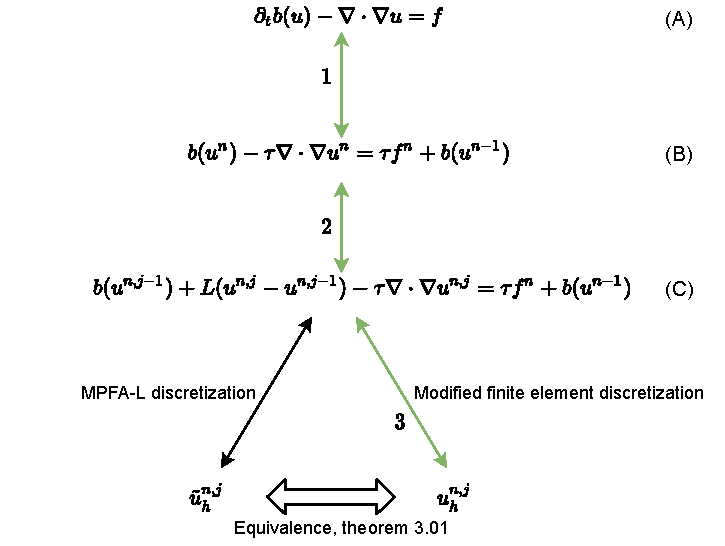
\includegraphics[width=0.8\textwidth]{convergence schema.pdf}
		\caption{}
		\label{fig:convergence schema}
	\end{figure}
	To prove convergence we list some assumptions:
	\begin{itemize}
		\item[\textbf{A-1}] The domain $\Omega\subset \mathbb{R}^2$ is bounded and have a Lipschitz continuos boundary, i.e., it is locally the graph of a Lipschitz continuous function.
		\item[\textbf{A-2}] $b\in C^1$ is non-decreasing and Lipschitz continuous.
		\item[\textbf{A-3}] $b(u_0)$ is essentially bounded in $\Omega$ and $u_0 \in L^2(\Omega)$.
	\end{itemize}
	\begin{theorem}
		Assume \textbf{A 1-3}, then
		Richards' equation after Kirchhoff transform \eqref{eq:richards simple} discretized with backward Euler in time, L-scheme linearization and MPFA-L discretization in space \eqref{eq:linearized richards fvm} converges, and we have the estimate
		\begin{equation}\label{eq:richards_estimate}
			\left \|\tilde{u}_h^{n}-u(t^n)\right \|_0 \leq C (h+\tau),
		\end{equation}
		where $C$ is some constant independent of the maximum mesh diameter $h$, the time step length $\tau$ and the minimum number of linearization iterations $j$.
	\end{theorem}
	\begin{proof}
		As the MPFA-L method and the modified finite element method are equivalent, we prove the convergence of our finite element solution, $u^{n,j}_h$.
		The proof will be done in three steps, see figure \ref{fig:convergence schema}.
		We have by the triangle inequality
		\begin{equation}
			\left \|u(t_n)-u_h^{n,j}\right \|_0 \leq\left \|u(t_n) -u^n  \right \|_0 + \left \|u^{n}-u^{n,j}\right \|_0 + \left \|u^{n,j}-u_h^{n,j}\right \|_0  .
		\end{equation}
		\begin{itemize}
			\item The third term is the error of solving the elliptic problem (C) in \ref{fig:convergence schema}, or 
			\begin{equation}\label{eq:first ineq}
				u^{n,j}-\frac{\tau}{L} \nabla \cdot \nabla u^{n,j} = \frac{L u^{n,j-1} + \tau f^n - b(u^{n,j-1}) + u^{n-1}}{L}.
			\end{equation}
			By theorem \ref{th:convergence of elliptic} we have the error estimate
			\begin{equation}
				\left \|u_h^{n,j}-u^{n,j}\right \|_1  \leq C h (\left \| u^{n,j-1} \right \|_2 + \left \| \frac{L u^{n,j-1} + \tau f^n - b(u^{n,j-1}) + u^{n-1}}{L} \right \|_0 + \left \| g \right \|_{\frac{1}{2},\Gamma_N}).
			\end{equation}
			The expression involving $u^{n-1}$ and $u^{n,j-1}$ are bounded independently of the mesh, see \cite{FlorinTimeConvergence} page 1459 for a stability estimate, hence $\left \|u_h^{n,j}-u^{n,j}\right \|_0 \leq C_3h$.
		\item To bound the second term, $\left \|u^{n,j}-u^n\right \|_0$, we will use techniques found in (Radu, List, \cite{list2016study}). First, we subtract the variational form of (B) from the variational form of (C) in figure \ref{fig:convergence schema}:
		For any $v\in H_0^1$ and $j>1$
		\begin{equation}\label{eq:L scheme 1}
			\left\langle b(u^{n,j-1})-b(u^n),v\right \rangle + \tau \left \langle \nabla (u^{n,j}-u^n), \nabla v\right \rangle +L\left \langle u^{n,j}-u^{n,j-1} ,v\right \rangle=0.
		\end{equation}
		Let $e^{n,j}:=u^{n,j}-u^n$, then test \eqref{eq:L scheme 1} with $e^{n,j}$:
		\begin{equation}
\left\langle b(u^{n,j-1})-b(u^n),e^{n,j}\right \rangle + \tau \left \| \nabla e^{n,j}\right \| +L\left \langle u^{n,j}-u^{n,j-1} ,e^{n,j}\right \rangle=0.
		\end{equation}
		Now, we use the relation $\left \langle b-a,b\right \rangle = \frac{1}{2}\left \|b\right\|^2+ \frac{1}{2}\left \|b-a\right\|^2-\frac{1}{2}\left \|a\right\|^2$ and some simple algebraic manipulation to obtain
		\begin{equation}
			\begin{aligned}
\left\langle b(u^{n,j-1})-b(u^n),e^{n,j-1}\right \rangle &+ \tau \left \| \nabla e^{n,j}\right \| + \frac{L}{2}\left \|e^{n,j}\right\|^2 + \frac{L}{2}\left \|e^{n,j}-e^{n,j-1}\right\|^2 \\ & \leq \frac{L}{2}\left \|e^{n,j-1}\right\|^2- \left\langle b(u^{n,j-1})-b(u^n),e^{n,j} - e^{n,j-1}\right \rangle.
			\end{aligned}
		\end{equation}
		Next, we use Cauchy Schwarz inequality on the first term, and Young's inequality on the last term
		\begin{equation}
			\begin{aligned}
&\left\| b(u^{n,j-1})-b(u^n)\right \| \left \|e^{n,j-1}\right \| + \tau \left \| \nabla e^{n,j}\right \| + \frac{L}{2}\left \|e^{n,j}\right\|^2 + \frac{L}{2}\left \|e^{n,j}-e^{n,j-1}\right\|^2 \\ & \leq \frac{L}{2}\left \|e^{n,j-1}\right\|^2 +\frac{1}{2L} \left\| b(u^{n,j-1})-b(u^n)\right\|^2+\frac{L}{2} \left \|e^{n,j} - e^{n,j-1}\right \|^2.				
\end{aligned}	
	\end{equation}
		We cancel the last term on the right side against the last term on the left side.
		Since $b(\cdot)$ is Lipschitz continuous with $\left \| b(x)-b(y)\right \| \leq L_B \left \|x-y\right \|$, we have
		\begin{equation}
			\begin{aligned}
				&\frac{1}{L_B}\left\| b(u^{n,j-1})-b(u^n)\right \|^2 + \tau \left \| \nabla e^{n,j}\right \| + \frac{L}{2}\left \|e^{n,j}\right\|^2  \\ & \leq \frac{L}{2}\left \|e^{n,j-1}\right\|^2 +\frac{1}{2L} \left\| b(u^{n,j-1})-b(u^n)\right\|^2.				
			\end{aligned}	
		\end{equation} 
		Using the Poincaré inequality we obtain
		\begin{equation}
			\left ( \frac{L}{2} + \frac{\tau}{C_{\Omega}} \right ) \left \|e^{n,j}\right \|^2 \leq \frac{L}{2} \left \|e^{n,j-1}\right \|^2+ \left ( \frac{1}{2L}-\frac{1}{L_B}\right ) \left \|b(u^{n,j-1})-b(u^n)\right \|^2.
		\end{equation}
		Since $L_B < 2L$ we reach the convergence estimate
		\begin{equation}
\left \|e^{n,j}\right \|^2 \leq \frac{L}{L+\frac{2\tau}{C_{\Omega}}}\left \|e^{n,j-1}\right \|^2
		\end{equation}
		Hence, $\left \| u^{n,j}-u^n\right \| = \left \| e^{n,j}\right \|\rightarrow 0$ as $j\rightarrow \infty$. Therefore, we choose $j$ such that
		\begin{equation*}
			\left \| u^{n,j}-u^n\right \|\leq (h+\tau), \ \ \forall n\in [1,N],
		\end{equation*}
		where $N=\lceil\frac{1}{\tau}\rceil $ is the number of time steps.
		\item The first term $\left \| u(t^n)-u^n\right \|$ can be bounded by the techniques used in (Radu, Pop and Knabner, \cite{FlorinTimeConvergence}). We reach the estimate
		\begin{equation}
			\left \| u^n-u(t^n)\right \|_0 \leq C_1 \tau.
		\end{equation}
		
		\end{itemize}
	Using all of the above, we get
	\begin{equation}
		\left \|\tilde{u}_h^{n}-u(t^n)\right \|_0 \leq C_3 h + C_1 \tau + \tau + h \leq (\max(C_1,C_3)+1)(h+\tau).
	\end{equation}
	We see from the above equation, that the desired result \eqref{eq:richards_estimate} is reached with $C=(\max(C_1,C_3)+1)$
	\end{proof}
	We have showed convergence for Richards' equation after Kirchhoff transform \eqref{eq:richards simple},  discretized in space by MPFA-L method, in time by backward Euler and L-scheme for linearization. In section \ref{sec:numerics_richards} we do numerical results to confirm this.
	\begin{remark}
		We expect that a better convergence rate estimate 
		\begin{equation}
			\left \|\tilde{u}_h^{n}-u(t^n)\right \|_0 \leq C (h^2+\tau),
		\end{equation}
		with the square of the mesh diameter, is possible. This is because we use the $\left\|\cdot\right\|_1$ estimate for the spatial discretization, but according to remark \ref{rem:l2_remark}, there exists a better $\left\|\cdot\right\|_0$ estimate we could use instead in the above proof.
	\end{remark}
	
\end{document}